\begin{example}{Implementation of a FSM}\label{ex:FSM}

\begin{figure}
  \begin{center}
    {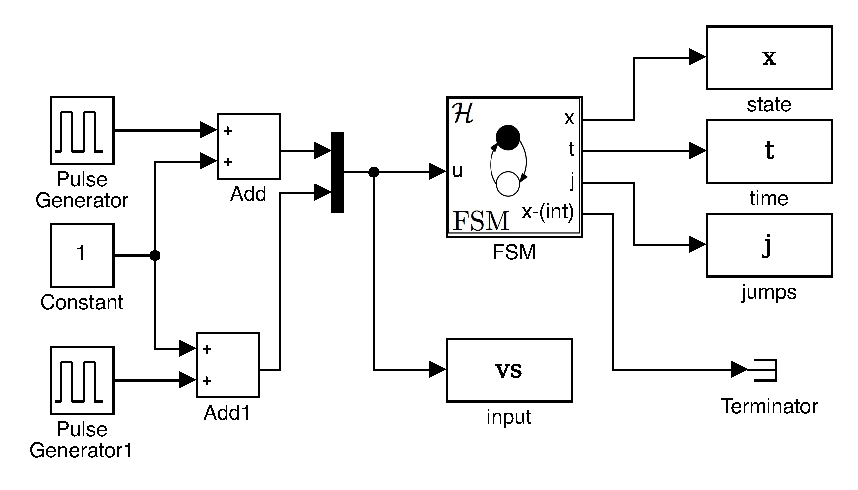
\includegraphics[width=0.6\textwidth]{figures/Simulink/FSM_example.eps}}
   \caption{Simulation of a Finite State Machine (FSM) in Example~\ref{ex:FSM}.}
\label{fig:FSM_example}
  \end{center}
\end{figure}

Transitions of the state of a FSM are triggered by changes of its input $\uc$.
The system can be modeled as a cascade of two systems,
in which an external signal drives the FSM. 
\IfSAE
{
A finite state machine (FSM) or deterministic finite automaton (DFA) is a system with
inputs, states, and outputs taking values from discrete sets that are updated at discrete transitions (or jumps)
triggered by its inputs. 
Then, given a FSM and an initial state $\xlogic_0 \in \xlogicSpace$,  
a transition to a state $\xlogic_1 = \delta(\xlogic_0,\uc)$ is performed
when an input $\uc \in \Sigma$ is applied to it.
After the transition, the output of the FSM is updated to $\hc(\xlogic_1)$.
This mechanism can be captured by the difference equation
\begin{eqnarray}\label{eqn:FSMmodel}
\xlogic^+ & = & \delta(\xlogic,\uc)  \qquad \yc \ = \ \hc(\xlogic) \qquad (\xlogic,\uc)  \in \xlogicSpace \times \Sigma
\end{eqnarray}
This model captures the dynamics
the model of the cyber components 
in the instructions document
with
$$
\xc = \xlogic, \qquad \xcSpace = \xlogicSpace, \qquad \ucSpace = \Sigma, \qquad \gc = \delta, \qquad \Dc = \xcSpace\times\ucSpace
$$
Note that there is no notion of time associated with the FSM model above. An example of this model is presented in Example~\ref{ex:FSM}. 
}
{The FSM is modeled as the difference equation in \eqref{eqn:FSMmodel}.}
Assuming that the input feeds the input $u$ of the FSM, 
the state of the FSM is updated according to the transition function evaluated at the current input, that is,
$\xlogic$ is updated according to
 $$
\xlogic^+  =  \delta(\xlogic,u)
$$

The above model can be summarized as follows:

\begin{align}\label{eqn:CTdynamicsHcFSM}
f(\xlogic, u)&:= \begin{bmatrix}0\\0\end{bmatrix},\\ 
   C :=& \defset{(\xlogic,u)\in\{1,2\}\times\{1,2\}\times\{1,2\}\times\{1,2\}}{ \delta(\xlogic,u) =  \xlogic},\\
g(\xlogic, u)&:= \delta(\xlogic, u) = \begin{bmatrix}3-u_1\\3-u_2\end{bmatrix}, \\
    D :=& \defset{(\xlogic,u)\in\{1,2\}\times\{1,2\}\times\{1,2\}\times\{1,2\}}{ \delta(\xlogic,u) \in\{1,2\}\times\{1,2\}\setminus \xlogic},\\ 
y &:= h(\xlogic) =\xlogic
\end{align}
where the input and the state are given by $u = (u_1,u_2) \in\{1,2\}\times\{1,2\}$, and $\xlogic=(\xlogic_1,\xlogic_2)\in\{1,2\}\times\{1,2\}$, respectively.

For the hybrid system FSM in Figure~\ref{fig:FSM_example} we have the following Matlab embedded functions that describe the sets $C$ and $D$ and functions $f$ and $g$.
Figure~\ref{fig:FSMresults} depicts the corresponding inputs and state of the FSM.

\begin{figure}[ht]
  \begin{center}
    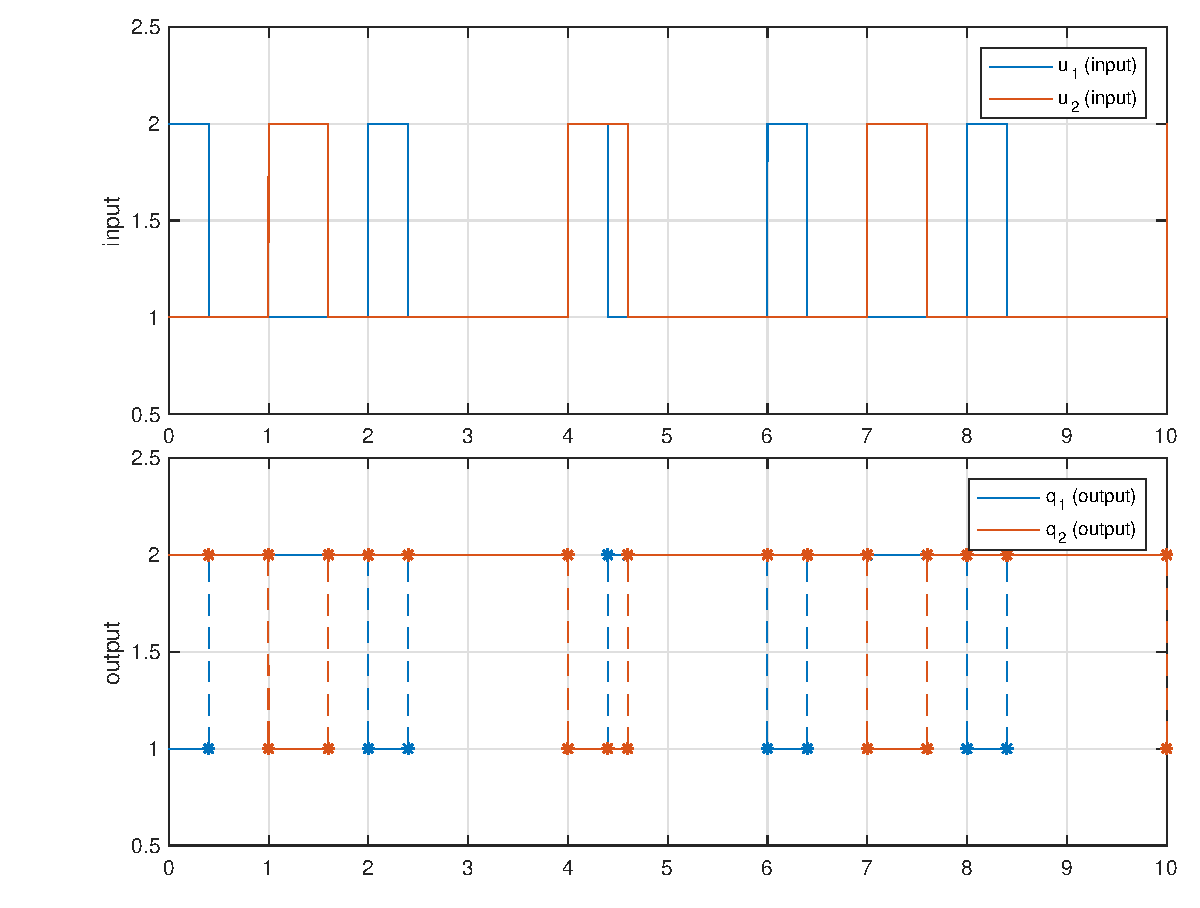
\includegraphics[width=0.8\textwidth]{figures/Simulink/FSMresults.eps}
   \caption{Finite state machine states and inputs.}
\label{fig:FSMresults}
  \end{center}
\end{figure}



Flow map
%\scriptsize
% This file was automatically created from the m-file 
% "m2tex.m" written by USL. 
% The fontencoding in this file is UTF-8. 
%  
% You will need to include the following two packages in 
% your LaTeX-Main-File. 
%  
% \usepackage{color} 
% \usepackage{fancyvrb} 
%  
% It is advised to use the following option for Inputenc 
% \usepackage[utf8]{inputenc} 
%  
  
% definition of matlab colors: 
\definecolor{mblue}{rgb}{0,0,1} 
\definecolor{mgreen}{rgb}{0.13333,0.5451,0.13333} 
\definecolor{mred}{rgb}{0.62745,0.12549,0.94118} 
\definecolor{mgrey}{rgb}{0.5,0.5,0.5} 
\definecolor{mdarkgrey}{rgb}{0.25,0.25,0.25} 
  
\DefineShortVerb[fontfamily=courier,fontseries=m]{\$} 
\DefineShortVerb[fontfamily=courier,fontseries=b]{\#} 
  
\noindent                    
 \hspace*{-1.6em}{\scriptsize 1}$  $\color{mblue}$function$\color{black}$ xdot = f(x, u, gamma)$\\
 \hspace*{-1.6em}{\scriptsize 2}$  $\\
 \hspace*{-1.6em}{\scriptsize 3}$  $\color{mgreen}#%%%%%%%%%%%%%%%%%%%%%%%%%%%%%%%%%%%%%%%%%%%%%%%%%%%%%%%%%%%%%%%%%%%%%%%%%%%#\color{black}$$\\
 \hspace*{-1.6em}{\scriptsize 4}$  $\color{mgreen}$% Matlab Function  Author: Ricardo Sanfelice $\color{black}$$\\
 \hspace*{-1.6em}{\scriptsize 5}$  $\color{mgreen}$% (Revised by Giampiero Campa)$\color{black}$$\\
 \hspace*{-1.6em}{\scriptsize 6}$  $\color{mgreen}$% (Revised by Pablo Nanez)$\color{black}$$\\
 \hspace*{-1.6em}{\scriptsize 7}$  $\color{mgreen}$%$\color{black}$$\\
 \hspace*{-1.6em}{\scriptsize 8}$  $\color{mgreen}$% Project: Simulation of a hybrid system (Bouncing Ball)$\color{black}$$\\
 \hspace*{-1.6em}{\scriptsize 9}$  $\color{mgreen}$%$\color{black}$$\\
 \hspace*{-2em}{\scriptsize 10}$  $\color{mgreen}$% Name: f.m$\color{black}$$\\
 \hspace*{-2em}{\scriptsize 11}$  $\color{mgreen}$%$\color{black}$$\\
 \hspace*{-2em}{\scriptsize 12}$  $\color{mgreen}$% Description: Flow map$\color{black}$$\\
 \hspace*{-2em}{\scriptsize 13}$  $\color{mgreen}$%$\color{black}$$\\
 \hspace*{-2em}{\scriptsize 14}$  $\color{mgreen}$% Version: 1.0$\color{black}$$\\
 \hspace*{-2em}{\scriptsize 15}$  $\color{mgreen}$% Required files: - $\color{black}$$\\
 \hspace*{-2em}{\scriptsize 16}$  $\color{mgreen}#%%%%%%%%%%%%%%%%%%%%%%%%%%%%%%%%%%%%%%%%%%%%%%%%%%%%%%%%%%%%%%%%%%%%%%%%%%%#\color{black}$$\\
 \hspace*{-2em}{\scriptsize 17}$  $\\
 \hspace*{-2em}{\scriptsize 18}$  $\\
 \hspace*{-2em}{\scriptsize 19}$  $\color{mgreen}$% flow map: xdot=f(x,u);$\color{black}$$\\
 \hspace*{-2em}{\scriptsize 20}$  xdot = [x(2); gamma];$\\ 
  
\UndefineShortVerb{\$} 
\UndefineShortVerb{\#}\label{scr:f}
%\normalsize

Flow set
%\scriptsize
% This file was automatically created from the m-file 
% "m2tex.m" written by USL. 
% The fontencoding in this file is UTF-8. 
%  
% You will need to include the following two packages in 
% your LaTeX-Main-File. 
%  
% \usepackage{color} 
% \usepackage{fancyvrb} 
%  
% It is advised to use the following option for Inputenc 
% \usepackage[utf8]{inputenc} 
%  
  
% definition of matlab colors: 
\definecolor{mblue}{rgb}{0,0,1} 
\definecolor{mgreen}{rgb}{0.13333,0.5451,0.13333} 
\definecolor{mred}{rgb}{0.62745,0.12549,0.94118} 
\definecolor{mgrey}{rgb}{0.5,0.5,0.5} 
\definecolor{mdarkgrey}{rgb}{0.25,0.25,0.25} 
  
\DefineShortVerb[fontfamily=courier,fontseries=m]{\$} 
\DefineShortVerb[fontfamily=courier,fontseries=b]{\#} 
  
\begin{Verbatim}[commandchars=\$\{\},numbers=left,numbersep=2pt] 

    $textcolor{mblue}{function} v  = C(x, u)  
     
    $textcolor{mgreen}{%%%%%%%%%%%%%%%%%%%%%%%%%%%%%%%%%%%%%%%%%%%%%%%%%%%%%%%%%%%%%%%%%%%%%%%%%%%} 
    $textcolor{mgreen} 
    $textcolor{mgreen} 
    $textcolor{mgreen} 
    $textcolor{mgreen} 
    $textcolor{mgreen}{% Version: 1.0} 
    $textcolor{mgreen}{% Required files: - } 
    $textcolor{mgreen}{%%%%%%%%%%%%%%%%%%%%%%%%%%%%%%%%%%%%%%%%%%%%%%%%%%%%%%%%%%%%%%%%%%%%%%%%%%%} 
     
    $textcolor{mgreen}{% state} 
    xi1 = x(1); 
    xi2 = x(2); 
     
    $textcolor{mgreen}{%input} 
    y2 = u(1); 
    v11 = u(2); 
    v12 = u(3); 
     
    $textcolor{mblue}{if} (xi1 >= y2)  $textcolor{mgreen}{% flow condition} 
        v = 1;  $textcolor{mgreen}{% report flow} 
    $textcolor{mblue}{else} 
        v = 0;   $textcolor{mgreen}{% do not report flow} 
    $textcolor{mblue}{end}  
\end{Verbatim}  
  
\UndefineShortVerb{\$} 
\UndefineShortVerb{\#} 
 \label{scr:C}
%\normalsize

Jump map
%\scriptsize
% This file was automatically created from the m-file 
% "m2tex.m" written by USL. 
% The fontencoding in this file is UTF-8. 
%  
% You will need to include the following two packages in 
% your LaTeX-Main-File. 
%  
% \usepackage{color} 
% \usepackage{fancyvrb} 
%  
% It is advised to use the following option for Inputenc 
% \usepackage[utf8]{inputenc} 
%  
  
% definition of matlab colors: 
\definecolor{mblue}{rgb}{0,0,1} 
\definecolor{mgreen}{rgb}{0.13333,0.5451,0.13333} 
\definecolor{mred}{rgb}{0.62745,0.12549,0.94118} 
\definecolor{mgrey}{rgb}{0.5,0.5,0.5} 
\definecolor{mdarkgrey}{rgb}{0.25,0.25,0.25} 
  
\DefineShortVerb[fontfamily=courier,fontseries=m]{\$} 
\DefineShortVerb[fontfamily=courier,fontseries=b]{\#} 
  
\noindent                    
 \hspace*{-1.6em}{\scriptsize 1}$  $\color{mblue}$function$\color{black}$ xplus = g(x, u)$\\
 \hspace*{-1.6em}{\scriptsize 2}$  $\color{mgreen}$% state$\color{black}$$\\
 \hspace*{-1.6em}{\scriptsize 3}$  xi = z(statevect);$\\
 \hspace*{-1.6em}{\scriptsize 4}$  xi1 = xi(1);      $\color{mgreen}$%x-position$\color{black}$$\\
 \hspace*{-1.6em}{\scriptsize 5}$  xi2 = xi(2);      $\color{mgreen}$%y-position$\color{black}$$\\
 \hspace*{-1.6em}{\scriptsize 6}$  xi3 = xi(3);      $\color{mgreen}$%orientation angle$\color{black}$$\\
 \hspace*{-1.6em}{\scriptsize 7}$  q = xi(4);$\\
 \hspace*{-1.6em}{\scriptsize 8}$  $\color{mgreen}$% q = 1 --> going left$\color{black}$$\\
 \hspace*{-1.6em}{\scriptsize 9}$  $\color{mgreen}$% q = 2 --> going right$\color{black}$$\\
 \hspace*{-2em}{\scriptsize 10}$  xi1plus=xi1;$\\
 \hspace*{-2em}{\scriptsize 11}$  xi2plus=xi2;$\\
 \hspace*{-2em}{\scriptsize 12}$  xi3plus=xi3;$\\
 \hspace*{-2em}{\scriptsize 13}$  qplus=q;$\\
 \hspace*{-2em}{\scriptsize 14}$  $\color{mgreen}$% jump map$\color{black}$$\\
 \hspace*{-2em}{\scriptsize 15}$  $\color{mblue}$if$\color{black}$ ((xi1 >= 1) && (q == 2)) || ((xi1 <= -1) && (q == 1))$\\
 \hspace*{-2em}{\scriptsize 16}$     qplus = 3-q;$\\
 \hspace*{-2em}{\scriptsize 17}$  $\color{mblue}$else$\color{black}$$\\
 \hspace*{-2em}{\scriptsize 18}$      qplus = q;$\\
 \hspace*{-2em}{\scriptsize 19}$  $\color{mblue}$end$\color{black}$$\\
 \hspace*{-2em}{\scriptsize 20}$  xplus = [xi1plus;xi2plus;xi3plus;qplus];$\\ 
  
\UndefineShortVerb{\$} 
\UndefineShortVerb{\#}\label{scr:g}
%\normalsize

Jump set
%\scriptsize
% This file was automatically created from the m-file 
% "m2tex.m" written by USL. 
% The fontencoding in this file is UTF-8. 
%  
% You will need to include the following two packages in 
% your LaTeX-Main-File. 
%  
% \usepackage{color} 
% \usepackage{fancyvrb} 
%  
% It is advised to use the following option for Inputenc 
% \usepackage[utf8]{inputenc} 
%  
  
% definition of matlab colors: 
\definecolor{mblue}{rgb}{0,0,1} 
\definecolor{mgreen}{rgb}{0.13333,0.5451,0.13333} 
\definecolor{mred}{rgb}{0.62745,0.12549,0.94118} 
\definecolor{mgrey}{rgb}{0.5,0.5,0.5} 
\definecolor{mdarkgrey}{rgb}{0.25,0.25,0.25} 
  
\DefineShortVerb[fontfamily=courier,fontseries=m]{\$} 
\DefineShortVerb[fontfamily=courier,fontseries=b]{\#} 
  
\noindent       
 \hspace*{-1.6em}{\scriptsize 1}$  $\color{mblue}$function$\color{black}$ v = D(x, u)$\\
 \hspace*{-1.6em}{\scriptsize 2}$  $\color{mgreen}$% jump set$\color{black}$$\\
 \hspace*{-1.6em}{\scriptsize 3}$  $\color{mblue}$if$\color{black}$ (x(1) <= u(1)) && (x(2) <= 0)  $\color{mgreen}$% jump condition$\color{black}$$\\
 \hspace*{-1.6em}{\scriptsize 4}$      v = 1;  $\color{mgreen}$% report jump$\color{black}$$\\
 \hspace*{-1.6em}{\scriptsize 5}$  $\color{mblue}$else$\color{black}$$\\
 \hspace*{-1.6em}{\scriptsize 6}$      v = 0;   $\color{mgreen}$% do not report jump$\color{black}$$\\
 \hspace*{-1.6em}{\scriptsize 7}$  $\color{mblue}$end$\color{black}$$\\ 
  
\UndefineShortVerb{\$} 
\UndefineShortVerb{\#}\label{scr:D}
%\normalsize


\end{example}
